\documentclass[a4paper, titlepage, 11pt, twocolumn] {article}
\usepackage{../of2}
%
\usepackage{tcolorbox}[all]
\usepackage{blindtext}
\usepackage{pdflscape}
\usepackage{array}
\usepackage{calc}
\usepackage{tikz}
\usepackage{eso-pic}
\usetikzlibrary{arrows.meta}

\tcbuselibrary{skins}
\graphicspath{..}

\begin{document}

\newcommand{\ofcssubtext}[2]{%
	\raisebox{-.1cm}{%
	\parbox[l]{\widthof{#1}}{%
		#1\vspace*{-0.2cm}\\
		{\scriptsize\acc{#2}}
	}
	}
}

\newcommand{\ofcsbox}[2]{%
	\begin{tcolorbox}[width=\columnwidth, boxrule=0.00cm, height=#1cm, sharp corners, colback=white, before skip=0cm, after skip=0pt, left=0mm,top=0pt,right=0mm,bottom=0pt, colframe=white]
	#2	
	\end{tcolorbox}
}

\newcommand{\ofcsinvisbox}[2]{%
	\begin{tcolorbox}[width=\columnwidth, boxrule=0.00cm, height=#1cm, sharp corners, colback=white, before skip=0cm, after skip=0pt, left=-3pt,top=-3pt,right=-3pt,bottom=-3pt, colframe=white]
		#2	
	\end{tcolorbox}
}

\newcommand{\ofcslimitbar}[0]{
	\raisebox{-.05cm}{%
	\tikz{
		\tikzstyle{seg}=[thick, draw, rectangle, align=center, minimum height = 0.35cm, minimum width = 0.6cm]
		\newcommand{\ofcslimitdist}{0.6}
		\node[seg](l0)at (0,0) {};					
		\node[seg](l1)at (\ofcslimitdist,0) {};
		\node[seg](l2)at (2*\ofcslimitdist,0) {};					
		\node[seg](l3)at (3*\ofcslimitdist,0) {};
		\node[seg](l4)at (4*\ofcslimitdist,0) {};
		\node[seg](l5)at (5*\ofcslimitdist,0) {};
		\node[seg](l6)at (6*\ofcslimitdist,0) {};					
		\node[seg](l7)at (7*\ofcslimitdist,0) {};
		\node[seg](l8)at (8*\ofcslimitdist,0) {};
		\node[seg](l9)at (9*\ofcslimitdist,0) {};
	}	
	}
}

\newcommand{\ofcsrulea}{\color{accent}\hspace*{-0.9cm}\rule{1.09\columnwidth}{2pt}}
\newcommand{\ofcsicon}[1]{\raisebox{-.1\height}{\includegraphics[height=0.7\baselineskip]{./art/icons/#1.png}}\hspace*{0.15cm}}

\newcommand{\ofcstest}[1]{	
	
	\AddToShipoutPictureBG*{%
		\begin{tikzpicture}[overlay,remember picture]
		%\draw[color=accent, line width=2pt]($ (current page.north west) + (0.035cm,-0.035cm) $)rectangle($ (current page.south east) + (-0.035cm,0.035cm) $);
		\draw[color=accent, line width=3pt]($ (current page.north west) + (0.053cm,-0.053cm) $)rectangle($ (current page.south east) + (-0.053cm,0.053cm) $);
		%\draw[color=accent, line width=1.5pt]($ (current page.north west) + (0.25cm,-0.25cm) $)rectangle($ (current page.south east) + (-0.25cm,0.25cm) $);
		\end{tikzpicture}
	}

	\newgeometry{bottom=0mm,top=4mm,right=6mm,left=6mm, columnsep=8mm}
	\thispagestyle{empty}
	\options{/cs,#1}
	\onecolumn
	\large
	%
	\begin{multicols}{3}
		\begin{tcolorbox}[enhanced, text fill, width=\columnwidth, boxrule=0.00cm, height=6cm, sharp corners, colback=white, before skip=0cm, after skip=0pt, left=0mm,top=0pt,right=0mm,bottom=0pt, colframe=white]			
			\accf{Name:}\hspace*{0.2cm}\option{/cs/name} \hfill
			\accf{Level:}\hspace*{0.1cm}\option{/cs/level}\\
			\option{/cs/description}\vfill
			\ofcssubtext{Talent:}{Level 2} \option{/cs/talent} 
		\end{tcolorbox}
		\ofcsbox{6}{
			\begin{center}
				\vspace*{-0.2cm}
				{\LARGE \accf{Character}\hspace*{0.25cm}\accf{Sheet}} \vspace*{0.5cm}\\
				
\includegraphics[width=0.55\columnwidth]{./art/images/ff9.jpg}
			\end{center}
		}
		\ofcsbox{6}{
			\accf{Story:}\\\option{/cs/story}
		}
	\end{multicols}
	%
	{\vspace*{-0.6cm}\ofcsrulea}\vspace*{-0.7cm}\\
	%
	\begin{multicols}{2}
	\ofcsbox{4.5}{
		\setlength{\columnsep}{0.7cm}
	\begin{multicols}{2}	
		\ofcsinvisbox{1.5}{
			\hspace*{\fill}\oficonhp\acc{H}ealth \acc{P}oints:\hspace*{\fill}\hspace*{0.8cm}\vspace*{-0.15cm}\\
			\hspace*{0.25cm}\hspace*{\fill}{\scriptsize\acc{current}\hspace*{0.3cm}\phantom{|}\hspace*{0.3cm}\acc{maximum}}\hspace*{\fill}\hspace*{0.8cm}\\
			\hspace*{\fill}\option{/cs/hpcur}\hspace*{0.4cm}|\hspace*{0.4cm}\option{/cs/hpmax}\hspace*{\fill}\hspace*{0.8cm}\\
		}
		\columnbreak
		\ofcsinvisbox{1.5}{
			\hspace*{\fill}\oficonmp\acc{M}ana \acc{P}oints:\hspace*{\fill}\hspace*{1cm}\vspace*{-0.15cm}\\
			\hspace*{0.25cm}\hspace*{\fill}{\scriptsize\acc{current}\hspace*{0.3cm}\phantom{|}\hspace*{0.3cm}\acc{maximum}}\hspace*{\fill}\hspace*{1cm}\\
			\hspace*{\fill}\option{/cs/mpcur}\hspace*{0.4cm}|\hspace*{0.4cm}\option{/cs/mpmax}\hspace*{\fill}\hspace*{1cm}\\
		}
	\end{multicols}
	%
	\vspace*{-0.8cm}
	%
	\begin{multicols}{2}
		\ofcsinvisbox{2.5}{
			\strnew\acc{STR}ength:\hfill\option{/cs/str}\hspace*{1cm}\ofrow
			\defnew\acc{DEF}ense:\hfill\option{/cs/def}\hspace*{1cm}\ofrow
			\magnew\acc{MAG}ic:\hfill\option{/cs/mag}\hspace*{1cm}\ofrow
			\resnew\acc{RES}istance:\hfill\option{/cs/res}\hspace*{1cm}
		}
		\columnbreak
		\ofcsinvisbox{2.5}{
			\oficonagi \acc{AGI}lity:\hfill\option{/cs/agi}\hspace*{1.3cm}\ofgap
			\ofcssubtext{Movement:}{= 1 + Agility}\hfill\option{/cs/movement}\hspace*{1.3cm}\ofgap
			\ofcssubtext{Evasion DC:}{= 12 - Agility}~\hfill\option{/cs/evasiondc}\hspace*{1.3cm}
		}
	\end{multicols}
	}	
	%
	\vspace*{-0.1cm}
	\ofcsbox{0.25}{Status Effects: \option{/cs/status}}
	%
	\columnbreak
	%
	\ofcsbox{4.5}{
		\ofcssubtext{Job:\phantom{yy}}{Level 1}\option{/cs/job}\hfill
		\ofcssubtext{Archetype:}{Level 3} \option{/cs/archetype}\vspace*{0.5cm}\\
		Special Abilities: \option{/cs/specials}\vspace*{0.6cm}\\
		Spells \& Techs:\ofrow \option{/cs/abilities}
	}
	\end{multicols}
	%
	{\vspace*{-0.4cm}\ofcsrulea}\vspace*{-0.7cm}\\
	%
	\begin{multicols}{2}
	\ofcsbox{3.8}{
		\ofcssubtext{Limit Break:}{Level 4} \option{/cs/limitbreak} \ofgap 
		Limit Mode: \option{/cs/limitmode}\ofrow
		Limit Points: \option{/cs/limitpoints}\hspace*{0.2cm}\ofcslimitbar\ofrow	
		\option{/cs/limitdesc}
	}
	\columnbreak
	\ofcsbox{3.8}{
		\ofcssubtext{Summon:}{Level 5}\option{/cs/summon}\ofgap
		Support: \option{/cs/summonsupport}	\ofrow
		Ability: \hfill {\small \acc{Cost: 10\% of current HP \& MP} \hfill \acc{Time: 1r}} \ofrow \option{/cs/summonability}
	}
	\end{multicols}
	%
	{\vspace*{-0.4cm}\ofcsrulea}\vspace*{-0.7cm}\\
	%	
	\begin{multicols}{2}
	\ofcsbox{5.1}{
		Weapon: \option{/cs/weapon}\\
		Effect: \option{/cs/weaponeffect}\\
		Materia: \option{/cs/weaponmateria}\ofrow
		Armor: \option{/cs/armor}\\
		Effect: \option{/cs/armoreffect}\\
		Materia: \option{/cs/armormateria}\ofrow			
		Accessory: \option{/cs/accessory1}\\
		Effect: \option{/cs/accessory1effect}\ofrow
		Accessory: \option{/cs/accessory2}\\
		Effect: \option{/cs/accessory2effect}
	}
	\columnbreak
	\ofcsbox{5.1}{
		Inventory:\hfill Gil:\hspace*{0.5cm}\option{/cs/gil}\\
		\option{/cs/inventory}
	}
	\end{multicols}
	%
	{\vspace*{-0.4cm}\ofcsrulea}\vspace*{-0.9cm}\\
	%
	\begin{multicols}{2}
	\hspace*{-0.3cm}
	\parbox{1.03\columnwidth}{
		\scriptsize
		\hfill\accf{Combat Actions Summary:}\hfill\ofrow
		\acc{Attack:} Attack with your weapon.
		Target makes an evasion check with DC 12 minus his AGI.
		On failure, the damage dealt is your weapon's DMG plus your STR.
		You score a critical hit (2x damage) if check is a 2.
		The target makes a counter attack if check is a 12.\ofrow
		\acc{Magic:} Cast a spell by spending MP, choosing a target in range and concentrating.
		While concentrating, you cannot take actions or evade. 
		After the cast time is up, the spell takes effect on the target right before your turn and cannot be evaded even if you are not in range anymore.
		If the spell deals damage or restores HP, add your MAG to the amount.\ofrow
		\acc{Tech:}
		Same as Magic but add your STR instead of MAG to damage and healing if bonus is not already included.\ofrow
		\acc{Defend:} Damage that you receive by Attacks until your next turn is halved. \ofrow
		\acc{Item:} Use an Item from your inventory on yourself or someone within 1u.\ofrow
		\acc{Re-Equip:} Swap a Materia or Equipment piece that you are wearing against one from your Inventory.\ofrow
		\acc{Dash:} Move another distance of your AGI+1 units.
	}
	\columnbreak\\
	\parbox{1.03\columnwidth}{
		\scriptsize	
		\hfill\accf{Status Effects Summary:}\hfill\ofrow
		\kosmall\accr{KO:} You are unconscious and your turns are skipped.\ofrow
		\blindsmall\accr{Blind}: On Attack, enemy has Advantage on the evasion check. \ofrow
		\poisonsmall\accr{Poison}: You take damage equal to 10\% of your maximum HP at the start of each turn, but cannot fall below 1 HP due to this effect.\ofrow
		\slowsmall\accr{Slow}: During your turn, you can either move or take an action but not both.\ofrow
		\sleepsmall\accr{Sleep}: You can't move or take actions. Removed when you take damage.\ofrow
		\zombiesmall\accr{Zombie}: All healing effects are reversed for you.\ofrow
		\silencesmall\accr{Silence}: You cannot begin casting Magic or using Techs.\ofrow
		\immobilesmall\accr{Immobile}: You are unable to move. \ofrow
		\destrsmall\dedefsmall\demagsmall\deressmall\accr{DeATR}: The attribute is reduced by 3, e.g. DeMAG reduces MAG. \ofrow
		\blinksmall\accg{Blink}: You have advantage on evasion checks. \ofrow
		\hastesmall\accg{Haste}: You can either make an additional action or movement. \ofrow
		\regensmall\accg{Regen}: Regain 10\% of your maximum HP at the start of each turn.\ofrow
		\enstrsmall\enndefsmall\enmagsmall\enressmall\accg{EnATR}: The attribute is increased by 3, e.g. EnMAG increases MAG. \ofrow
	}
	\end{multicols}
}
\ofcstest{limitpoints=}
\ofcstest{
	name=Lightning,
	%
	description={%
		\vspace*{-0.5cm}
		\begin{multicols}{2}
			Age: 21\\Race: human\\Hair: rose\\Height: 1.70m\\Right-Handed\ofrow Personality:\\Determined\\ Cold
			\columnbreak\\
			\hspace*{-0.4cm}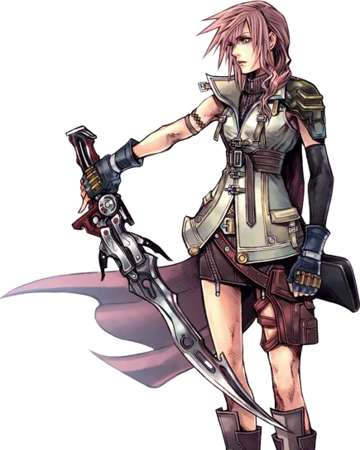
\includegraphics[width=1.5\columnwidth]{./art/images/claire.jpg}
		\end{multicols}
		\vspace*{-0.9cm}
	},
	%
	story={\vfill
		Both of my parents died when I was young. 
		I raised my sister Serah and joined the army where I became a sergeant. 
		But now Serah is in danger so I have quit the army to find her. 
		\\\\
		"It's not a question of can or can't. There are some things in life you just do."
	},
	% 
	hpcur=17, hpmax=99, mpcur=13, mpmax=71, agi=3, movement=4u, evasiondc=9, str=6, def=3, mag=5, res=3, 
	%
	level=8, job=Red Mage, archetype=Ravager, talent=Guardian Corps,
	%
	abilities={Cure, Fire, Blizzard, Thunder, Blind,\\ Poison, Esuna, NulElement},
	specials={Overwhelm, Swiftcast}, status={Blind (1r), EnDEF (2r)},
	%
	limitbreak=Thundara, limitmode=Brave, limitrange=5u, limittarget=2u, 
	limitdesc={A barrage of lightning strikes descends upon an enemy within 5u and everyone within 2u of him. All affect targets suffer 2d+8 lightning damage.},
	%
	summon=Odin, summonused=yes, summonsupport={Conjure horse Sleipnir}, summonability={Target on the battlefield suffers KO with DC~8 check or 3 times Level damage otherwise.},
	%
	weapon=Gunblade (Expert), weaponeffect=Ranged attack after ability, armor=Guardian Corps Uniform, armoreffect=DEF~+1, accessory1=Power Armlet, accessory1effect=STR~+1,
	%
	gil=2009, inventory={\\Survival Knife, 5x Bomb Fragment, 5x Hi-Potion\\ 3x Remedy, 2x Phoenix Down, 1x Elixir}
}
	%
\clearpage
%
\end{document}